\chapter{SVG feature representation}
Our goal is to extend beyond polyline modeling and capture the higher-level shapes of SVG objects.
Thus, our first challenge is to choose an adequate representation that captures all drawing information from an SVG and can be fed as an input vector to our neural network architecture.
Although many different elements are allowed by the SVG specification, we simplify the problem space to focus only on \code{path}s (since \code{path}s can be used to compose other elements anyway). 

\section{Overview of SVG commands}
There are five commands possible in an SVG \code{path}~\cite{grasso2011svg}:

\begin{enumerate}
    \item \textbf{Move}: moves the pen to a specified position (\code{m dx dy})
    \item \textbf{Line}: draws a line from the start to the end position (\code{l dx dy})
    \item \textbf{Cubic B\'ezier}: draws a cubic curve according to given control points (\code{c dx1 dy1, dx2 dy2, dx dy})
    \item \textbf{Quadratic B\'ezier}: draws a quadratic curve according to given control point (\code{q dx1 dy1, dx dy})
    \item \textbf{Arc}: draws a section of an ellipse (\code{a rx ry x-axis-rotation large-arc-flag sweep-flag dx dy})
\end{enumerate}

For simplicity, the above enumeration omits the absolute coordinate variants of the previous commands, which specify absolute $(x, y)$ coordinates instead of relative $(dx, dy)$.

\section{Modeling SVGs}
We would like to model SVG inputs without loss of information about pen movements.
In essence, since SVGs name ordered lists of paths and their drawing commands, we model them as a sequence of mathematical parameters for the pen drawing commands and add a command for representing the transition between paths.
The sequential nature of this representation makes the generation task well-suited to a recurrent neural network architecture, as we cover in Chapter~\ref{chap:architecture}.

\subsection{Preprocessing}
SVG icons and font glyphs often have additional properties like stroke and fill style.
As we focus on path generation exclusively, our first step in transforming input SVGs is to strip away those styles and focus only on the \code{path} elements of the input, often resulting in an image that depicts the outlines of the input shape---see Figure~\ref{fig:input_fonts} for examples.

Often, designers do not craft SVGs by editing XML by hand but rather with interactive image editing software such as Adobe Illustrator or Inkscape (\TODO{citations?}).
Thus, human-created SVGs often have varying path compositions, viewboxes, and canvas sizes.

To constrain the generation process slightly, we first homogenize our dataset by preprocessing inputs to rescale to the same overall canvas size (set to $256\times 256$ pixels) as well as reorder paths in the drawing sequence so that paths with larger bounding boxes are drawn first.

There is also variability in the direction of path drawing and in starting positions. Instead of controlling these factors in the preprocessing stage, our architecture is designed for bidirectionality, and all command sequences are prepended such that the pen starts at coordinate $(0, 0)$.

\subsection{Simplifying path commands}
As seen in our dataset statistics in Sections~\ref{sec:icon-data} and~\ref{sec:font-data}, the most common SVG path command used in our input data is the cubic B\'ezier drawing command, \code{c}, by a large margin.
To avoid bias and to constrain the problem space (\TODO{wording?}), we instead consolidate the different path commands into a single feature representation.

Out of the five SVG path commands, three are parametic equations of differing degrees, so we can model these three (lines, quadratic B\'eziers, and cubic B\'eziers) using the parameter space for the highest degree cubic-order equation.
An elliptical arc segment, on the other hand, cannot be perfectly transformed into a cubic B\'ezier. Arcs have five extra parameters used to describe them ($x$-radius, $y$-radius, angle of rotation, the large arc flag, and the sweep flag), but they occur relatively rarely in the dataset, so it makes sense to approximate them with the same parameter space as used for our parametric commands.
We use the following method to approximate arc segments as cubic B\'eziers (further mathematical explanation can be found in Appendix~\ref{app:convert-arc}).

\begin{enumerate}
    \item Extract the arc parameters: start coordinates, end coordinates, ellipse major and minor radii, rotation angle from $x$ and $y$ axes, large arc flag, and sweep flag. 
    \item Transform ellipse into unit circle by rotating, scaling, and translating, and save those transformation factors.
    \item Find the arc angle from the transformed start point to end point on the unit circle.
    \item If needed, split the arc into segments, each covering an angle less than $90^\circ$.
    \item Approximate each segment angle's arc on a unit circle such that the distance from the circle center to the arc along the angle bisector of the arc is equal to the radius, defining cubic B\'ezier control points.
	\item Invert the transformation above to convert arcs along the unit circle back to the elliptical arc, transforming the generated control points accordingly.
	\item Use these transformed control points to parameterize the output cubic B\'ezier curve.
\end{enumerate}

After all path drawing command types have been transformed to use the parameters needed for modeling cubic B\'ezier segments, we can represent each SVG command as a feature vector comprising those parameters and a three-dimensional one-hot pen state vector, similar to the feature representation used in~\cite{ha2017neural}.

In all, our feature representation models each drawing command as a nine-dimensional vector (in contrast to the five-dimensional feature vector for polyline drawings in~\cite{ha2017neural}).
Six dimensions are used to model three $x, y$ coordinate parameters of cubic B\'eziers, and three dimensions are reserved for the pen up, pen down, and end drawing pen states.
In the next section, we examine the details of this feature transformation process and how its tweaks affect modeling performance.

\section{Feature representation variability}
We find that alternative forms of this feature adaptation process have varying ``learnability'', as training variants of the transformed inputs with the same model architecture produces outputs of differing quality.

Some examples of variation are:
\begin{itemize}
\item \textbf{Absolute vs.\ relative coordinates}: are start, end, and control points represented in terms of their absolute position in the drawing or their relative displacement between each other?
\item \textbf{Coordinate system orientation}: if relative, do we specify displacement vectors in terms of the normal $\{(1, 0), (0, 1)\}$ basis, or do we transform their values such that they represent deviations from continuing in the same direction as the previous point?
\item \textbf{Pairwise coordinate choice}: if relative, between which points in the curves' coordinate parameters do we measure displacement?
\end{itemize}

\subsection{Encoding experiment}
To investigate the effects of choices for the above questions, we train five models each with a different feature encoding for input and output drawings.

\begin{table}[t]
\centering
\caption[Feature encoding variants]{The differences between the five feature representations used for the encoding efficacy experiment. Each feature encoding uses six dimensions for the cubic B\'ezier parameters (two for each point vector) and three for the pen state (pen up, pen down, end drawing). Note that \code{s} represents the start coordinates of the curve, \code{e} represents the end coordinates of the curve, \code{c1} represents the coordinates of the curve's first
control point, and \code{c2} represents the coordinates of the curve's second control point. \code{disp(a, b)} indicates displacement between points \code{a} and \code{b}, and \code{rot(v)} indicates that vector \code{v} has been applied a transformation to rotate its coordinate axes to be in the \TODO{direction of the previous vector in the encoding}.\label{tbl:features}}
\begin{minipage}[b]{\linewidth}
\begin{tabularx}{\linewidth}{c X}
\toprule
encoding & feature vector description \\ \midrule
A & \code{disp(s, e), disp(s, c1), disp(s, c2), pen\_state}\\
B & \code{disp(s, c1), disp(c1, c2), disp(c2, e), pen\_state}\\
C & \code{disp(s, e), rot(disp(s, c1)), rot(disp(c2, e)), pen\_state}\\
D & \code{e, rot(disp(s, c1)), rot(disp(c2, e)), pen\_state}\\
E & \code{e, c1, c2, pen\_state}\\
\end{tabularx}
\end{minipage}
\end{table}

All models are trained using the same architecture as described in Chapter~\ref{chap:architecture}, for \TODO{count} steps.
To generate the differently encoded inputs, the same base dataset of SVGs for the glyph ``b'' in various font faces is transformed to produce a set of feature vectors for each representation in Table~\ref{tbl:features}.
The base dataset is then partitioned randomly into 1920 training examples, 240 validation examples, and 240 test examples.
SVGs whose total number of path commands is greater than 250 are pruned.
Graphs depicting loss during the training process can be found in Appendix~\ref{app:train-encs}.

\subsubsection{Results}
For each of the models, the model iteration with the best validation loss is selected for evaluation.
Qualitative results from the encoding experiment can be found in Figure~\ref{fig:encodings}.

We evaluate results quantitatively by \TODO{eval!!!!}.

\begin{figure}[t]
	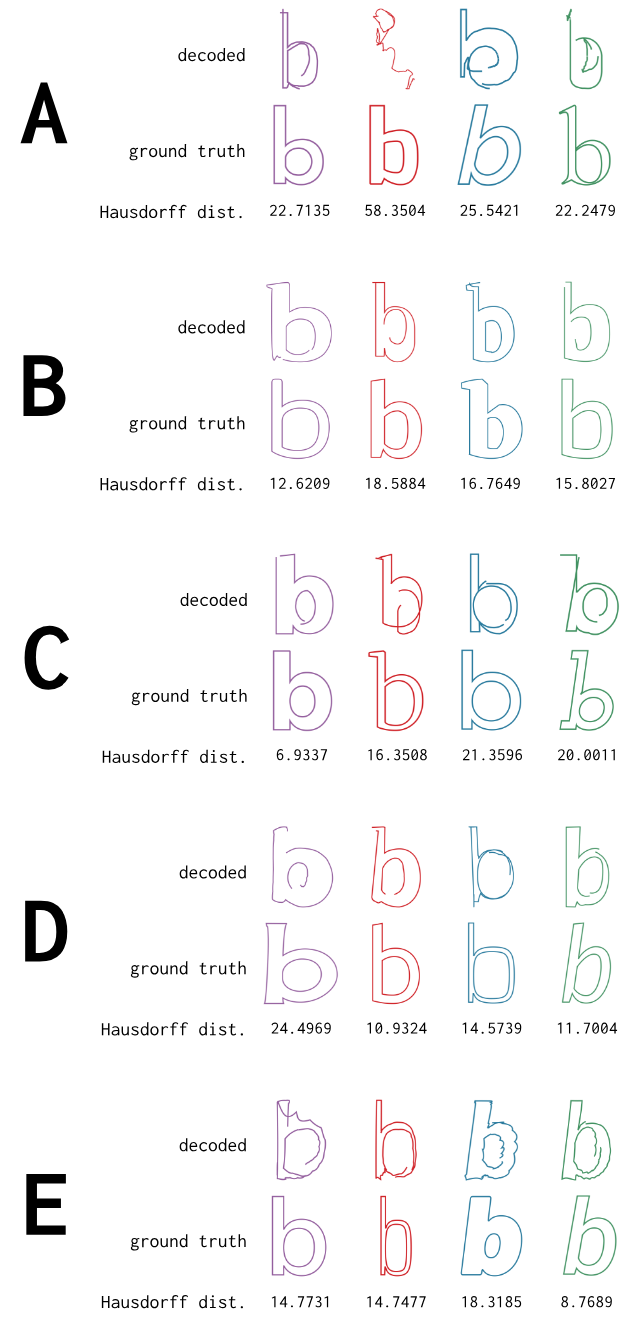
\includegraphics[width=\textwidth]{figures/encodings}
    \caption[Visual results of training the SVG model with different encodings]{Randomly sampled input-output pairs from the SVG models trained on the five encodings described in Table~\ref{tbl:features}. Decoded outputs were generated at temperature 0.3. Decoded outputs are found on the left, while ground truth inputs are on the right.\label{fig:encodings}}
\end{figure}
